\documentclass[thesis.tex]{subfiles}
\newcommand\TPR{\mathit{TPR}}
\newcommand\FPR{\mathit{FPR}}
\newcommand\OMP{\mathit{1-P}}
\newcommand\TP{\mathit{TP}}
\newcommand\FP{\mathit{FP}}
\newcommand\TN{\mathit{TN}}
\newcommand\FN{\mathit{FN}}
\newcommand\ROC{ROC}
\newcommand\PR{PR}

\begin{document}
\chapter{Image correspondence}
\label{sec:ic}

In this chapter we explain the image correspondence problem and the application of our descriptor to solve the problem.

The image correspondence problem is the problem of matching features across two images $A$ and $B$ of the same object. A match should ideally indicate that the two features correspond to the same physical point or object. The two images of the object can be captured under different lighting conditions, taken from different positions, and have varying tilt, rotation, zoom, and focus; hence the images will differ based on these variables. By using an interest point detector in combination with a descriptor, we are able to find interest points in $A$ and $B$, describe each interest point with a descriptor algorithm, and compare these descriptors across the two images by a given similarity measure to estimate whether the points match.

\section{Matching strategies}
\label{sec:matching_strategies}

The matching performance depends on the matching strategy. \citet{mikolajczyk2005performance} described the following three matching strategies that are used when solving the image correspondence problem:
Simple \emph{thresholding} compares each descriptor in image $A$ with each descriptor in image $B$. Any two descriptors having a mutual distance below a threshold $t$ are classified as matches (positive). \emph{Best-thresholding} finds the best matching descriptor in $B$ for each descriptor in $A$. If the distance is below a threshold $t$, it is a match (positive), and otherwise it is rejected (negative). \emph{Ratio-thresholding} finds the two best matching descriptors in $B$ with distances $B_1$ and $B_2$ for each descriptor in $A$. If the ratio between the two distances ($\frac{B_1}{B_2}$) to the descriptor in $A$ is below a threshold $t$, it is a match (positive). Otherwise the match is rejected (negative). In other words a distance ratio close to 0 is a good match.

We choose the ratio-thresholding strategy since this is the one favoured in previous image correspondence evaluations \cite{mikolajczyk2005performance,dahl2011finding,larsen2012jet,lowe2004distinctive}. Additionally this matching strategy is more general since it uses the ratio between the distance to the two best matching features instead of the absolute values giving less dependence on the descriptor in question. The two following cases give a good rationale for choosing this matching strategy: The first case is when two descriptors are good matches. In this case the descriptors will be very similar, and their difference could be caused by noise or other small variations. Due to this fact the algorithm shouldn't choose one over the other and hence the matching is negative since the distance ratio is close to 1. The second case is when only poorly matching descriptors are present. In this case the distance to both of the best matching descriptors will be high and the distance ratio close to 1 giving us a negative match as desired.


\section{Similarity measure}
\label{sec:similarity_measure}
We need a similarity measure in order to compute the distance between two descriptors. The Euclidean distance is widely used as similarity measure in the literature \cite{lowe2004distinctive,ke2004pca,mikolajczyk2005performance}. \citet{larsen2012in} evaluated the following different similarity measures: $L_1$ distance, Euclidean distance, $\chi^2$ distance, Kullback-Leibler divergence, and Jensen-Shannon divergence, and he found no notable difference in performance for his locally orderless-based descriptor. Based on this and some preliminary tests of our descriptor, where Euclidean distance ($L_2$) slightly outperformed $L_1$-distance, we choose to use Euclidean distance.

\section{Performance measures}
\label{sec:performance_measures}

Having established the matching strategy and similarity measure, we now describe the two performance measures which we use for evaluation of descriptor algorithms.

Assume that we have computed the descriptor distances, found the two best matching descriptors in $B$ for each descriptor in $A$ and computed their distance ratio $r$. We now wish to compute the performance of the descriptor algorithm utilized. The problem has been reduced to a binary classification problem of whether two descriptors match or not. Following the approach described in \Cref{sec:binaryClassificationMeasures}, using $r$ as the classification score $s$, we are able to compute the PR- and ROC-curves as well as their AUCs to get a measure of the performance of our descriptor.

Recall the discussion of the benefits of ROC and PR in \Cref{sec:binaryClassificationMeasures}. The PR measure is beneficial to use when the positive class is of greater importance than the negative class. In the image correspondence problem we wish to find as many corresponding points as possible and hence the PR measure has greater importance than the ROC measure. This however doesn't mean that it isn't important to be able to classify negatives.

%The approach is similar to that of \citet{winder2009picking,dahl2011finding}.

\section{Dataset}
The dataset we use for training and evaluation of our descriptor is called the \emph{DTU Robot 3D dataset} \cite{aanaes2010recall} (from now on called the DTU dataset). It consists of images of objects taken in a closed black box with varying illumination using 19 fixed position LED lights. In total there are 60 scenes with varying objects. \Cref{fig:dtu_examples} shows 4 example scenes. \citet{aanaes2010ground} classify the scenes into categories as shown in \Cref{tbl:dtu_scene_classifications}.

\begin{figure}[p]
	\centering
	\begin{subfigure}{0.49\textwidth}
		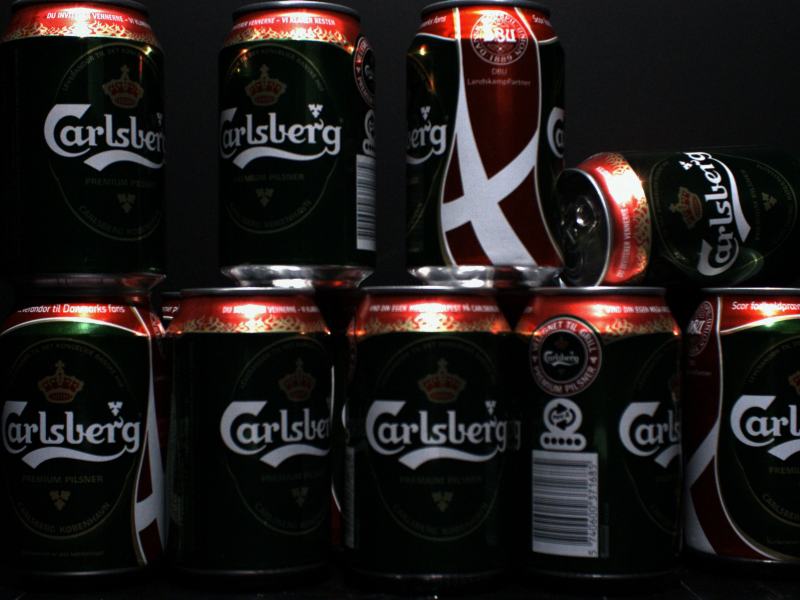
\includegraphics[width=\textwidth]{img/dtu_example_1.png}
	\end{subfigure}
	\hfill
	\begin{subfigure}{0.49\textwidth}
		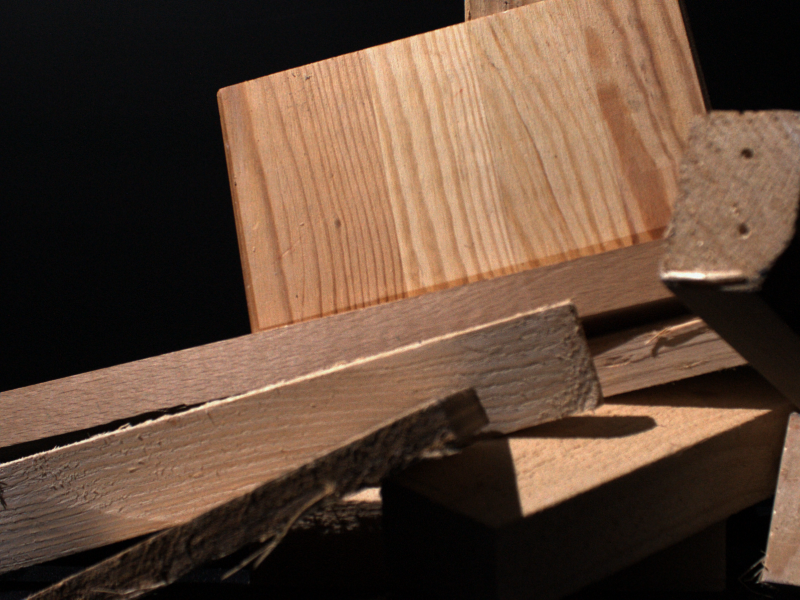
\includegraphics[width=\textwidth]{img/dtu_example_2.png}
	\end{subfigure}
	\par\medskip
	\begin{subfigure}{0.49\textwidth}
		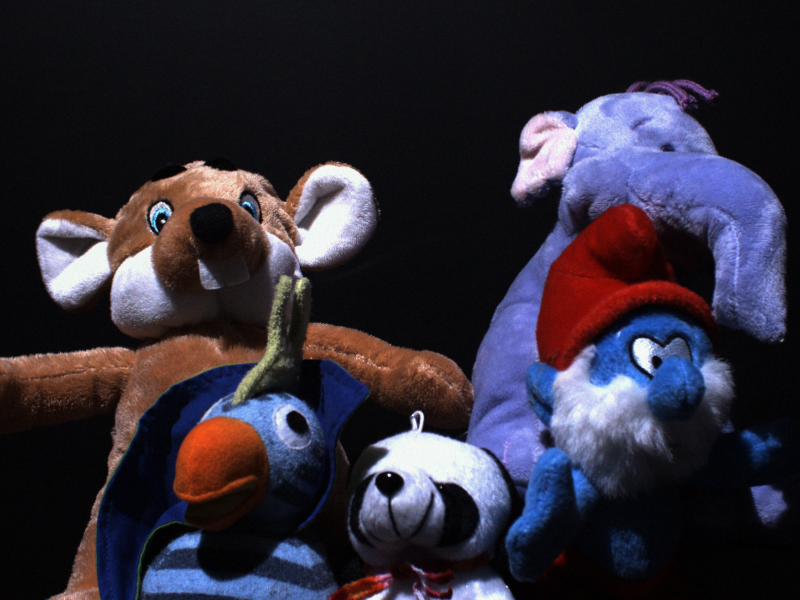
\includegraphics[width=\textwidth]{img/dtu_example_3.png}
	\end{subfigure}
	\hfill
	\begin{subfigure}{0.49\textwidth}
		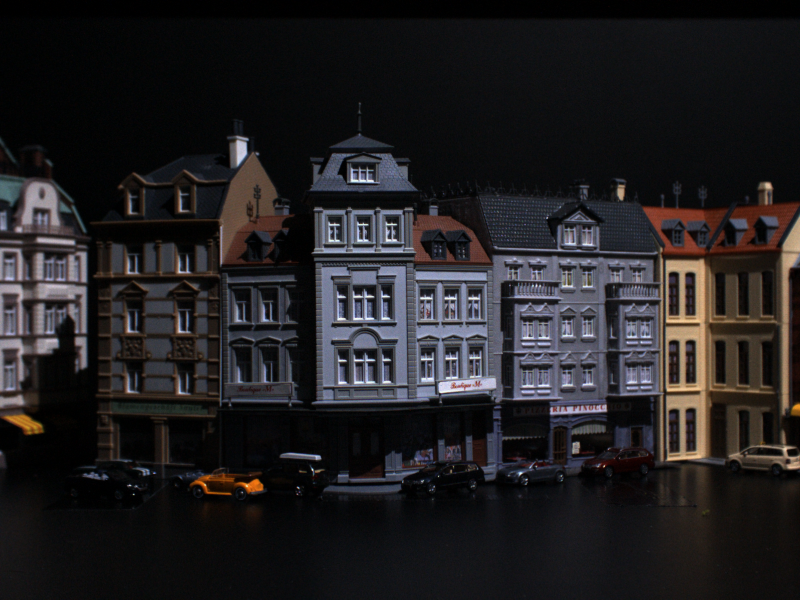
\includegraphics[width=\textwidth]{img/dtu_example_4.png}
	\end{subfigure}
	\caption{Example scenes from the DTU dataset}
	\label{fig:dtu_examples}
%
\vspace{1cm}
%
	\centering
	\begin{tabular}{l l r}
		\toprule
		Class & Scene numbers & Total \\
		\midrule
		House					& 1, 4, 8, 31, 32, 49, 50, 55				& 8 \\
		Books					& 2, 11, 20, 21								& 4 \\
		Fabric					& 5, 6, 45, 46, 47, 48						& 6 \\
		Greens					& 23, 24, 25, 26, 27, 51, 52, 53, 54, 56	& 10 \\
		Beer  					& 15, 16									& 2 \\
		Teddy Bears 			& 9, 10, 43, 44								& 4 \\
		Building Materials 		& 33, 34, 35, 36, 37						& 5 \\
		Decorative Items (Art) 	& 38, 39, 40, 41, 42						& 5 \\
		Groceries 				& 12, 28, 29, 30							& 4 \\
		Twigs and Leaves 		& 17, 57, 58, 59, 60 						& 5 \\
		\bottomrule
	\end{tabular}
	\caption{Scene object classifications from \cite[Table 1]{aanaes2010ground}}
	\label{tbl:dtu_scene_classifications}
\end{figure}

The camera is positioned around each scene using an industrial robot arm, which has automatically captured each scene from 119 positions. These positions are defined from a fixed frontal view varying the viewpoint $\theta$ in three arcs at different distance $d$ to the scene. Arc 1 has $d = \SI{0.5}{\meter}$ to the scene and $\theta$ spans $\SI{\pm40}{\degree}$, arc 2 has $d = \SI{0.65}{\meter}$ and $\theta$ spans $\SI{\pm25}{\degree}$, and arc 3 has $d = \SI{0.8}{\meter}$ and $\theta$ spans $\SI{\pm20}{\degree}$. Furthermore a linear path is captured by moving the camera away from the scene, which corresponds to zooming or scaling the scene. This is done at $\theta = \SI{0}{\degree}$ and $d$ spans $[\SI{0.5}{\meter};\SI{0.8}{\meter} ]$. At each of the 119 camera positions 19 individual images $I_i$ are taken with each of the LED lights $i,~\text{for}~i = 1,\hdots,19$ turned on. Using the given camera positions we get four camera paths: three arc paths and one linear path. \Cref{fig:dtu_overview} shows an overview of the four camera paths just described. When computing the performance across the paths we wish to solve the image correspondence problem for matching each image in each path with the \emph{keyframe} image (middle position on arc 1), since this gives us the performance when varying the viewing angle and scale in a structured manner.

\begin{figure}[tb]
	\centering
	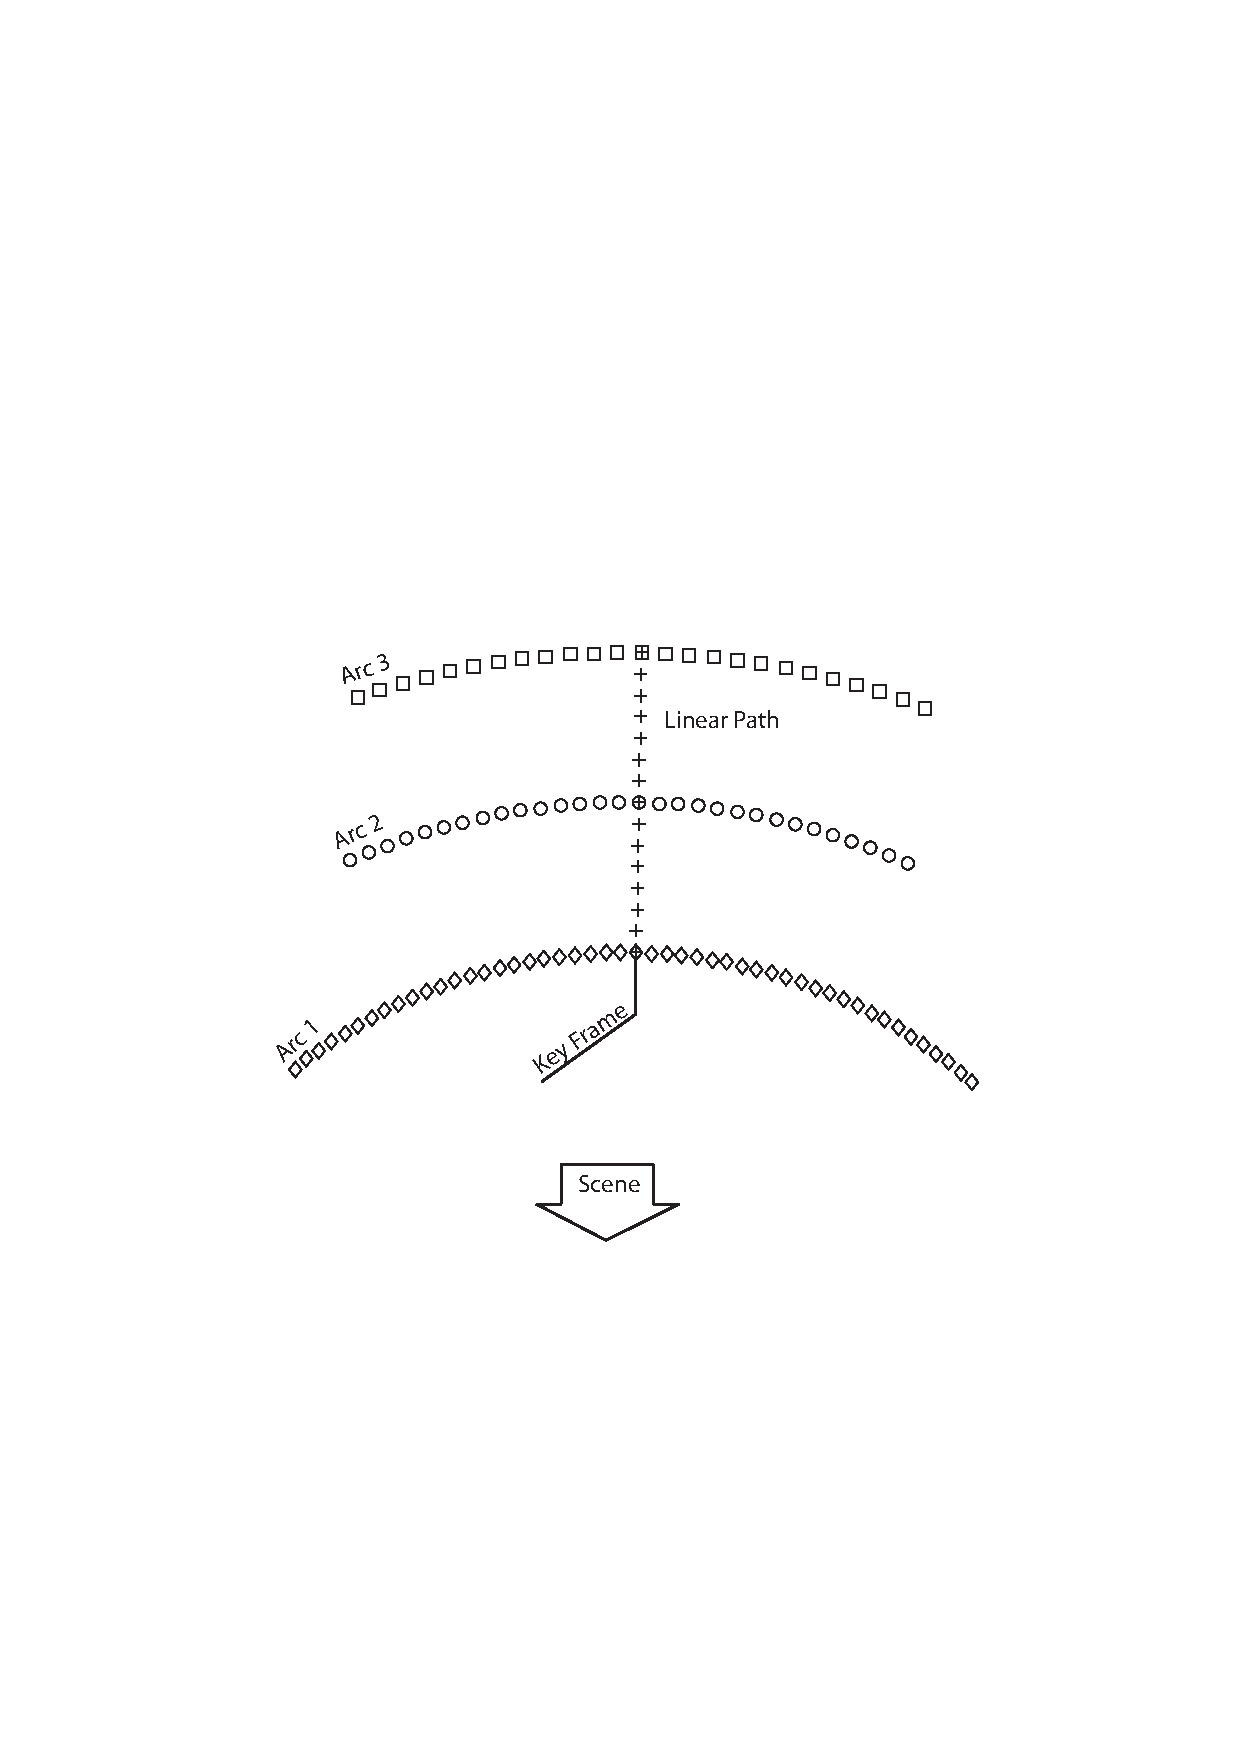
\includegraphics[width=0.8\textwidth]{img/CameraPosb.pdf}
	\caption{Overview of camera positions and paths in the DTU dataset. The figure originates from \cite{aanaes2010recall}.}
	\label{fig:dtu_overview}
\end{figure}

The choice of capturing the scenes with individual LED lights created images with a high amount of cast shadows. \citet{larsen2012jet} created a set\footnote{dataset available at http://roboimagedata.imm.dtu.dk/data/condensed.tar.gz} of artificial diffuse and light paths from the individual LED images which we now briefly explain. The artificial diffuse light images are created from the individual lightings in order to only evaluate the performance of our descriptor under viewpoint changes and to get more natural images. These diffuse images are created by averaging over the individual light images for each camera position:
\begin{align}
	I_{\text{diffuse}} = \frac{1}{19} \sum_{i = 1}^{19} I_{i}
\end{align}
Since the dataset consists of individual LED images, one is able to construct images simulating two light source paths going from right to left and back to front respectively.
Given a light position ${\boldsymbol{x}}$ in the spatial domain of the LED positions, the image $I_{\boldsymbol{x}}$ is constructed by weighting each LED image by the Gaussian of the distance to ${\boldsymbol{x}}$:
\begin{align}
	I_{x} = \sum_{i = 1}^{19} G(\boldsymbol{x} - \boldsymbol{x}_i,\sigma) I_{i}
\end{align}
In order to get a somewhat general measurement for the robustness against light variations there are light paths generated for the following four image positions: 12 (arc 1), 25 (arc 1), 60 (linear path), and 87 (arc 2).
See \citet{aanaes2010recall,aanaes2010ground} for more information about the dataset and the generated light paths.

\Cref{fig:light_example} show 6 of the different light images for scene 4 at camera position 60. \Cref{fig:light_example_02,fig:light_example_17,fig:light_example_08} show the images taken with individual LED lighting (numbers 2, 17, and 8 respectively), and \Cref{fig:light_example_00} shows the diffuse light image. We here notice the significant difference in cast shadows using the three LEDs individually compared to the diffuse light image. The diffuse light image is however quite dark compared to the LED 8 light image, which could potentially cause problems in some scenes generating too few interest points. Such an issue could however be handled by adapting detection thresholds or by using histogram stretching/equalization.
\Cref{fig:light_example_28,fig:light_example_20} show the left- and rightmost positions of the X light path. By comparing these to their LED counterparts (\subref{fig:light_example_02} and \subref{fig:light_example_17} respectively) we see that the cast shadows are less significant therefore looking more natural.
\Cref{fig:viewpoint_example} shows 4 different camera positions for scene 4 including the keyframe (position 25)..
%
\begin{figure}[tb]
	\centering
	\begin{subfigure}{0.49\textwidth}
		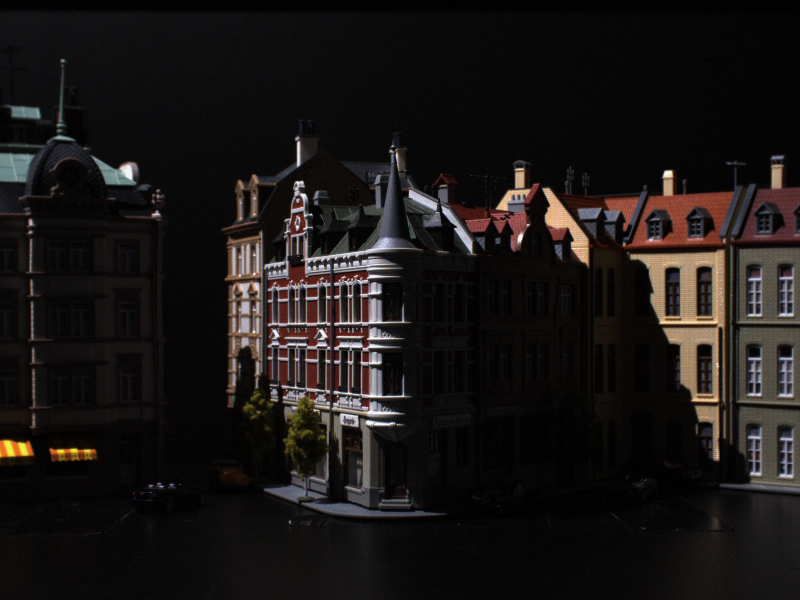
\includegraphics[width=\textwidth]{img/scene_04_img60_02.png}
		\caption{LED 2 light}
		\label{fig:light_example_02}
	\end{subfigure}
	\begin{subfigure}{0.49\textwidth}
		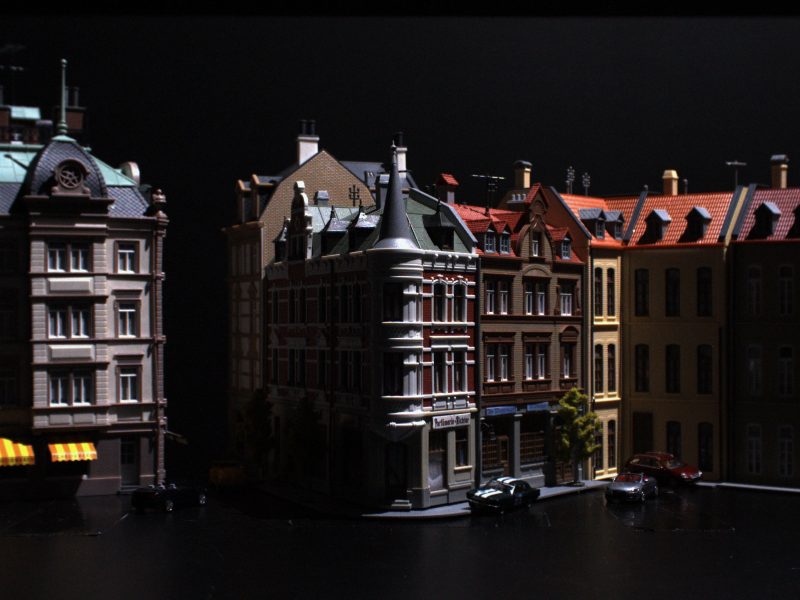
\includegraphics[width=\textwidth]{img/scene_04_img60_17.png}
		\caption{LED 17 light}
		\label{fig:light_example_17}
		\end{subfigure}
	\begin{subfigure}{0.49\textwidth}
		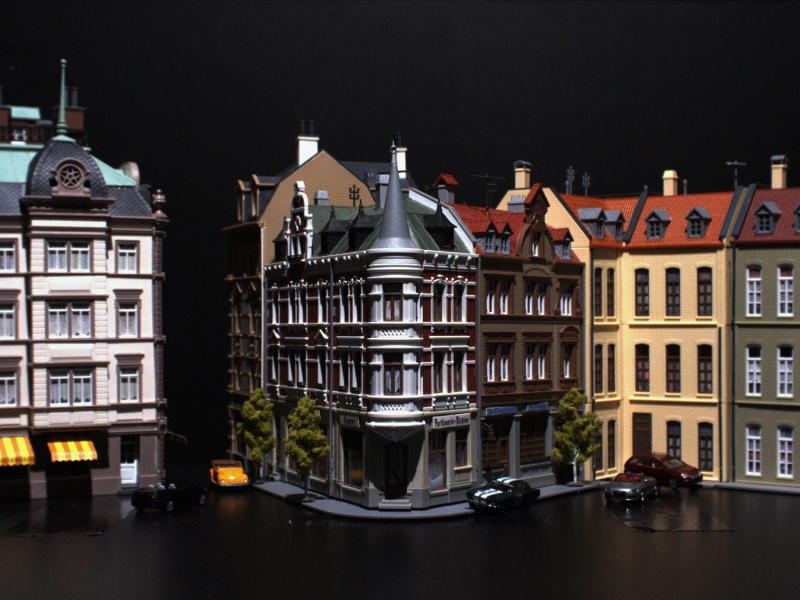
\includegraphics[width=\textwidth]{img/scene_04_img60_08.png}
		\caption{LED 8 light}
		\label{fig:light_example_08}
	\end{subfigure}
	\begin{subfigure}{0.49\textwidth}
		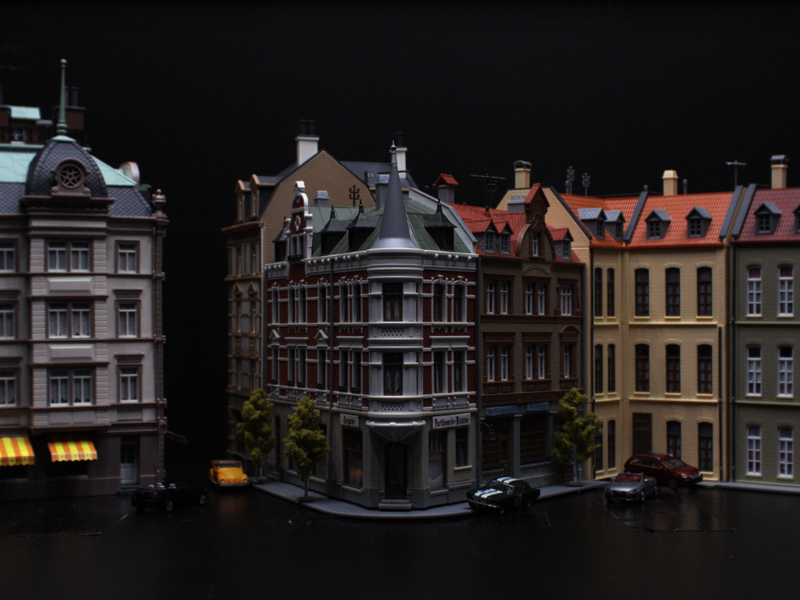
\includegraphics[width=\textwidth]{img/scene_04_img60_00.png}
		\caption{Diffuse light}
		\label{fig:light_example_00}
	\end{subfigure}
	\begin{subfigure}{0.49\textwidth}
		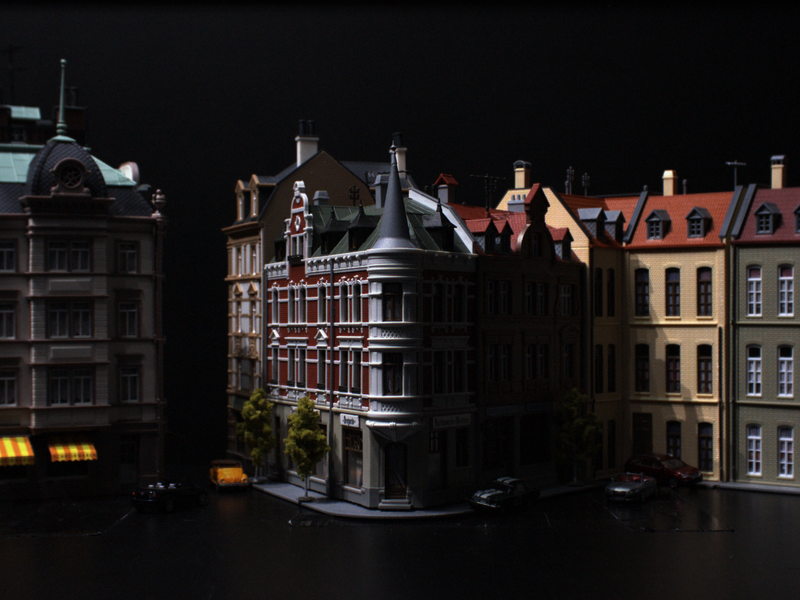
\includegraphics[width=\textwidth]{img/scene_04_img60_28.png}
		\caption{Leftmost position of X light path}
		\label{fig:light_example_28}
	\end{subfigure}
	\begin{subfigure}{0.49\textwidth}
		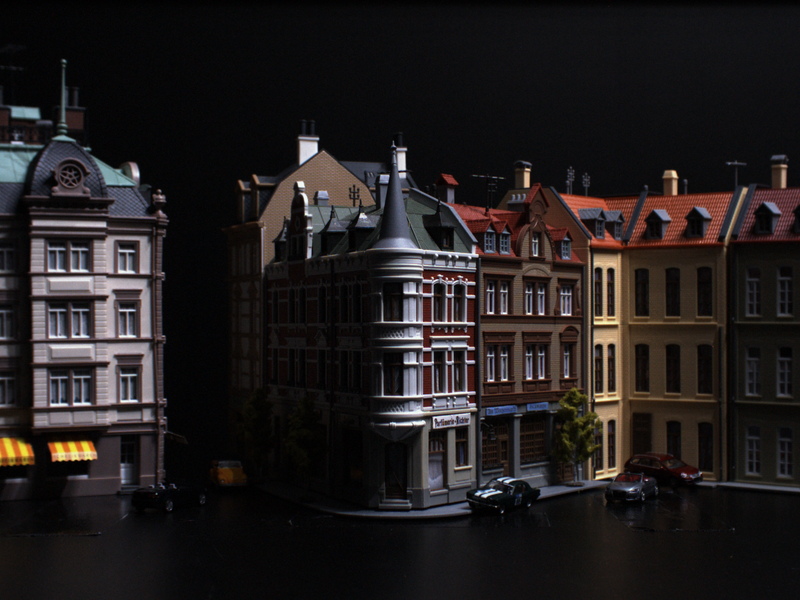
\includegraphics[width=\textwidth]{img/scene_04_img60_20.png}
		\caption{Rightmost position of X light path}
		\label{fig:light_example_20}
	\end{subfigure}
	\caption{Examples of light images in scene 4 at camera position 60.}
	\label{fig:light_example}
\end{figure}
%
\begin{figure}[tb]
	\centering
	\begin{subfigure}{0.49\textwidth}
		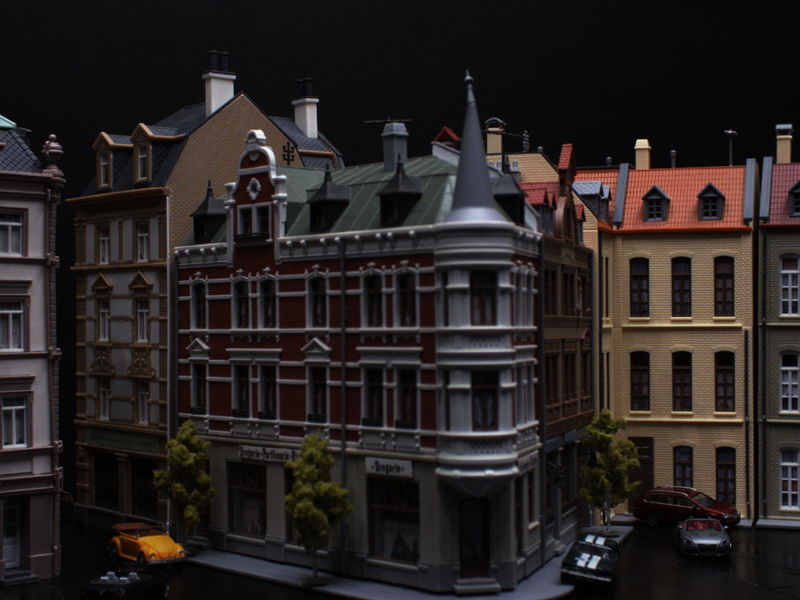
\includegraphics[width=\textwidth]{img/scene_04_img12_00.png}
		\caption{Camera position 12 (arc 1)}
		\label{fig:viewpoint_example_left}
	\end{subfigure}
	\begin{subfigure}{0.49\textwidth}
		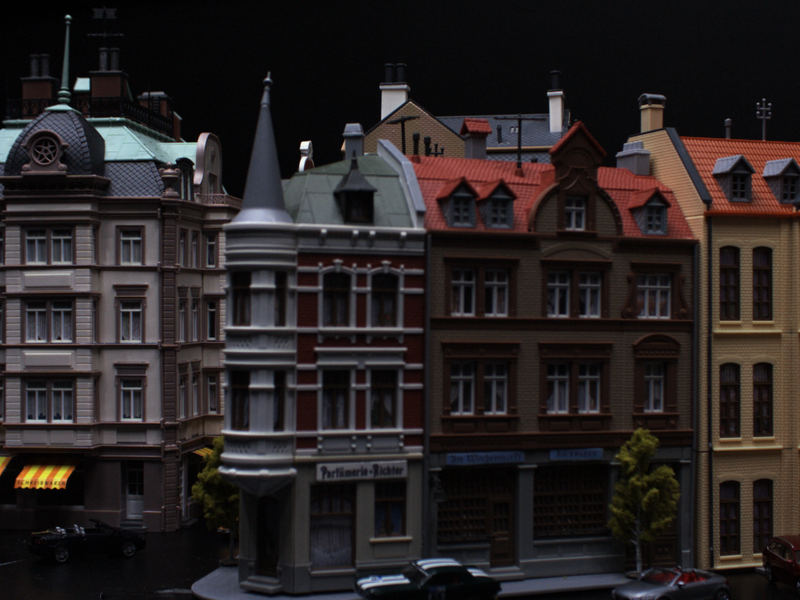
\includegraphics[width=\textwidth]{img/scene_04_img47_00.png}
		\caption{Camera position 47 (arc 1)}
		\label{fig:viewpoint_example_right}
	\end{subfigure}
	\begin{subfigure}{0.49\textwidth}
		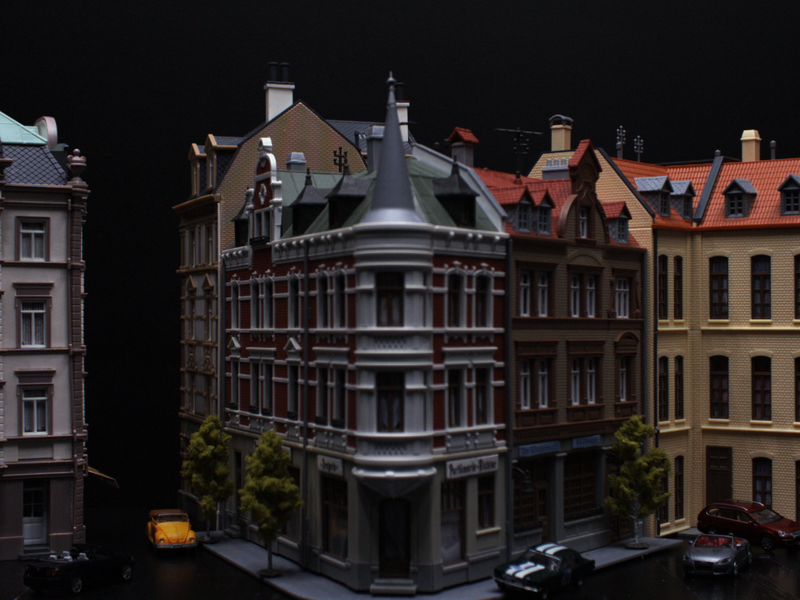
\includegraphics[width=\textwidth]{img/scene_04_img25_00.png}
		\caption{Camera position 25 (keyframe)}
		\label{fig:viewpoint_example_keyframe}
	\end{subfigure}
	\begin{subfigure}{0.49\textwidth}
		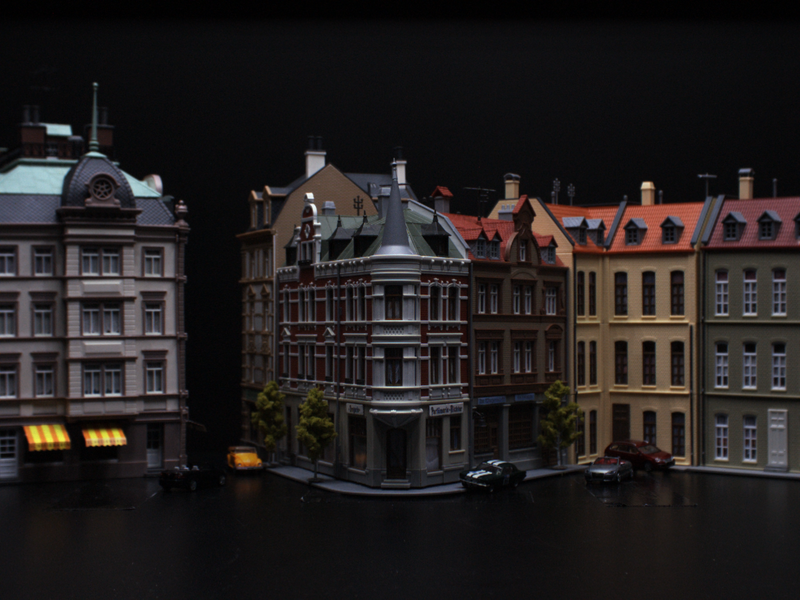
\includegraphics[width=\textwidth]{img/scene_04_img64_00.png}
		\caption{Camera position 64 (linear path)}
		\label{fig:viewpoint_example_scale}
	\end{subfigure}
	\caption{Examples of various camera positions of scene 4 using diffuse light.}
	\label{fig:viewpoint_example}
\end{figure}
%
\subsection{Evaluation}
In order to be able to classify matches between two images $A$ and $B$ as true or false, we need an evaluation method. In other words we need to compute/generate the match ground truth. The DTU dataset has been scanned using \emph{structured light} generating point clouds for the surfaces in each image. Using these points and the known camera positions for each image we are able to check if a matching of two points from $A$ and $B$ indeed correspond to 3D points close enough to one another to be true. \citet{aanaes2010recall} defined three evaluation criteria, of which we will be using the two first: Epipolar and surface geometry. We first define the property of being 3D reconstructable: an image point is said to be 3D reconstructable if there exists a point from the surface point cloud within a 10 pixel window in the image plane. This corresponds to a pixel within approximately 6 mm in the surface point cloud. Sometimes a matching is made for a point which is not 3D reconstructable. In this case no ground truth can be calculated, and the matching is ignored in the performance evaluation. The following two criteria (illustrated in \Cref{fig:icEvalGT}) determine the matching correspondence ground truth of the two points:
\begin{itemize}
	\item \textbf{Epipolar geometry consistency:} Given a point in the first image, the point in the second image should be within a 2.5 pixel orthogonal distance to the epipolar line of the first point as illustrated in \Cref{fig:icEval1GT}.
	\item \textbf{Surface geometry consistency:} The points need to be 3D reconstructable and they need to be within 3 mm of each other in the surface point cloud as illustrated in \Cref{fig:icEval2GT}.
\end{itemize}

\todo{Should we refer to \cite{larsen2012in}?}

\begin{figure}[tb]
	\centering
	\begin{subfigure}[t]{0.8\textwidth}
		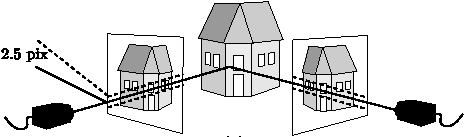
\includegraphics[width=\textwidth]{img/icEval1GT.pdf}
		\caption{Epipolar geometry consistency. Corresponding points should have an orthogonal distance to each others epipolar lines of maximum 2.5 pixel.}
		\label{fig:icEval1GT}
	\end{subfigure}
	\begin{subfigure}[t]{0.8\textwidth}
		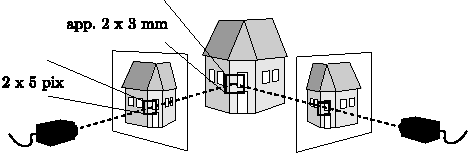
\includegraphics[width=\textwidth]{img/icEval2GT.pdf}
		\caption{Surface geometry consistency. Corresponding descriptors should be 3D reconstructable and be within 3 mm of each other in the surface point cloud.}
		\label{fig:icEval2GT}
	\end{subfigure}
	\caption{Illustration of the two ground truth evaluation criteria. Figure reproduced from \cite[Figure 5 (a-b),pp. 4]{aanaes2010recall}}
	\label{fig:icEvalGT}
\end{figure}

%
\subsection{Pitfalls and deficiencies}
The DTU dataset is built to test the ability of computer vision systems to cope with viewpoint changes, scaling, light changes, and to a certain extent occlusions as well. Since all images are captured with the same camera tilt, no rotation of objects occurs and hence rotational invariance and robustness cannot be evaluated using this dataset.

\Cref{fig:dtu_problems} shows the problems we have found within the DTU dataset, which we will go through here.

The artificial diffuse light is, as mentioned in the previous section, created by combining images captured under individual LED lighting. This is not optimal as some of the images are visually suffering from the spatial layout of the LED lights. \Cref{fig:dtu_problems_diffuse} shows image 20 (arc 1) from set 2 of the dataset. The diffuse light problem is clearly visible in the cast shadows seen on the 1st and 3rd book in the stack of lying books. Ideally these shadows would form either a smoothed or a single hard shadow edge instead of a number of gradually fading hard edges.

The automatic capturing of images using a robot arm combined with the individual LED lighting has the side-effect of the robot arm casting shadows in some of the images. This is seen when using the 3rd LED light and having captured the scenes from the far left of arc 1. \Cref{fig:dtu_problems_robot} shows an example of a cast shadow originating from the robot arm. This is however only a problem with one of the 19 LED light images and hence the effect on the final test images is minimal.
%
\begin{figure}[tb]
	\centering
	\begin{subfigure}{0.49\textwidth}
		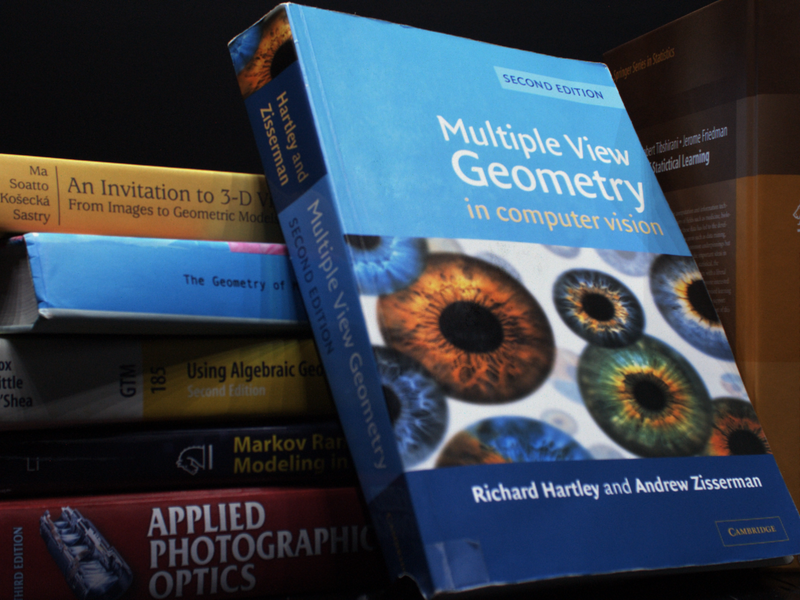
\includegraphics[width=\textwidth]{img/diffuse_light_problem.png}
		\caption{Diffuse lighting in set 2, image 20, with shadow artifacts}
		\label{fig:dtu_problems_diffuse}
	\end{subfigure}
	\begin{subfigure}{0.49\textwidth}
		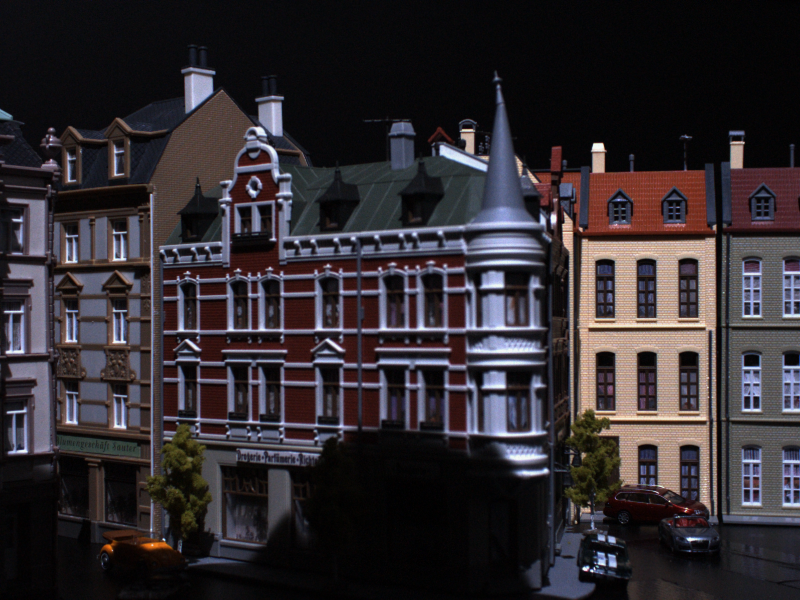
\includegraphics[width=\textwidth]{img/robot_arm_shadow.png}
		\caption{Robot arm shadow in set 4, image 7, LED light 3}
		\label{fig:dtu_problems_robot}
	\end{subfigure}
	\caption{Examples of problematic images in the DTU dataset}
	\label{fig:dtu_problems}
\end{figure}
%
\section{Example}
%
In this section we will continue the example from \Cref{sec:proposedDescriptorExample} by extending it to show the results of solving the image correspondence problem between the image of the example and the corresponding keyframe image from the DTU robot dataset.
\Cref{fig:imageCorrespondenceMatches} shows matches between the descriptors from the two images with score $s$ below threshold $t = 0.8$. The green and red lines indicate true and false positive classifications respectively. The images contain several similar beer cans and hence many of the false positive classifications are caused by patterns that are visible in multiple of the cans.

\Cref{fig:imageCorrespondenceCorrectMatch,fig:imageCorrespondenceIncorrectMatch} show two examples of a true positive match and a true negative match respectively. The green line shows a condition positive match and the red lines show condition negative matches. In \Cref{fig:imageCorrespondenceCorrectMatch} we see that there indeed is a correspondence between the best match of the two images with distance 0.083, and that our matching strategy results in a distance ratio (score) $s$ of 0.92. In \Cref{fig:imageCorrespondenceIncorrectMatch} we see that there is no match between the best matching descriptors of each image with distance 0.081. For this match $s$ is computed to 0.97. If we wanted to classify both matches correctly we should therefore set our threshold $t$ between 0.92 and 0.97. If we had used the distance as similarity measure we would not have been able to classify both correctly since the distance of the condition negative match is lower than the distance of the condition positive match.

When having computed the distance ratios of all matches, we are able to construct the ROC- and PR-curves giving us two measures of the performance of the descriptor matching. \Cref{fig:imageCorrespondenceCurves} shows the ROC-curve \subref{fig:imageCorrespondenceROC} and PR-curve \subref{fig:imageCorrespondencePR} as well as the area under the two curves. The match has a ROC AUC of 0.72 and PR AUC of 0.63. From the ROC plot wee see that the descriptor matching performs better than a random classification since the ROC-curve (blue line) lies above the curve of no predictive value (dashed line). This is likewise indicated by the ROC AUC which is above the random classification ROC AUC of 0.5.

\newgeometry{left=2cm,right=2cm,top=3cm,bottom=3cm}
\begin{figure}[p]
	\centering
	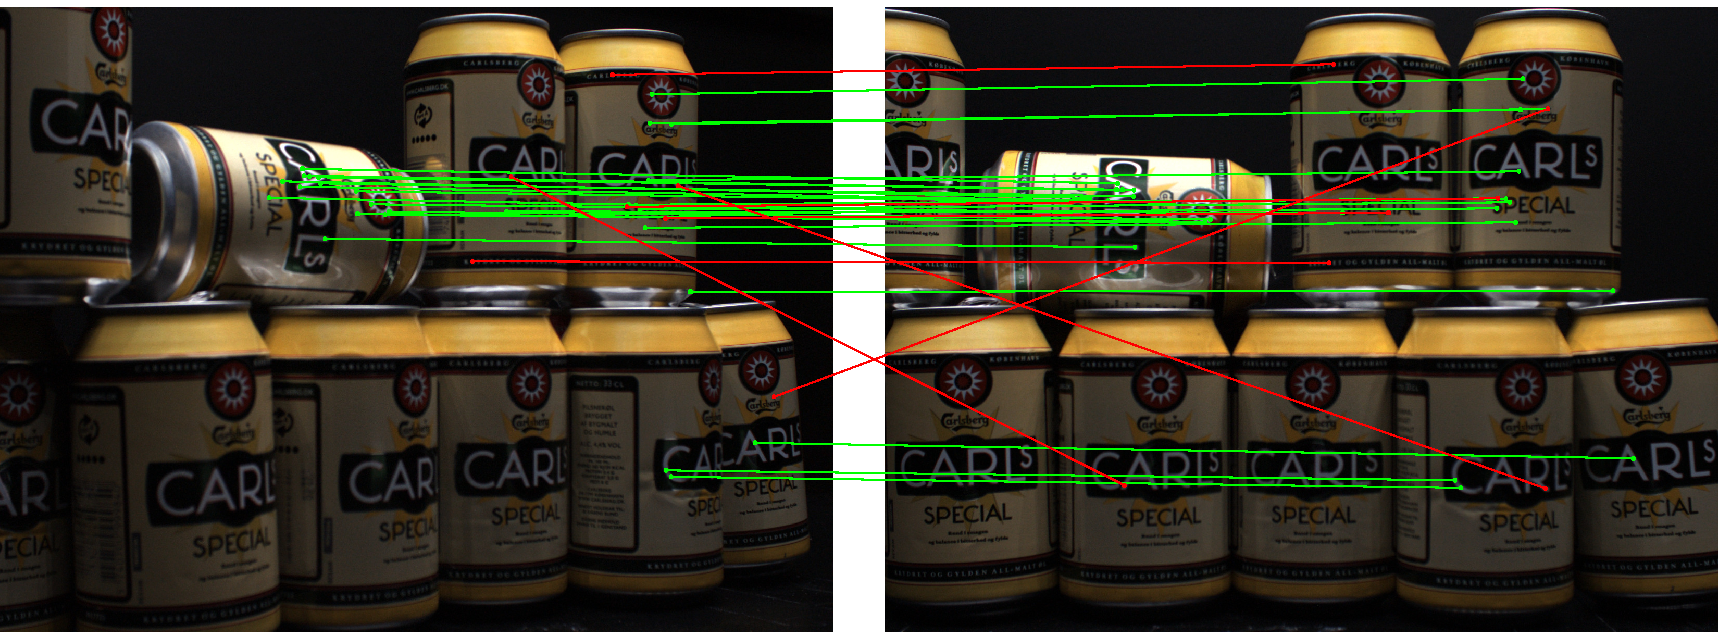
\includegraphics[width=\textwidth]{img/imageCorrespondenceMatches.pdf}
	\caption{Matches with score $s$ below threshold $t = 0.8$}
	\label{fig:imageCorrespondenceMatches}
	\vspace{5mm}
	%
	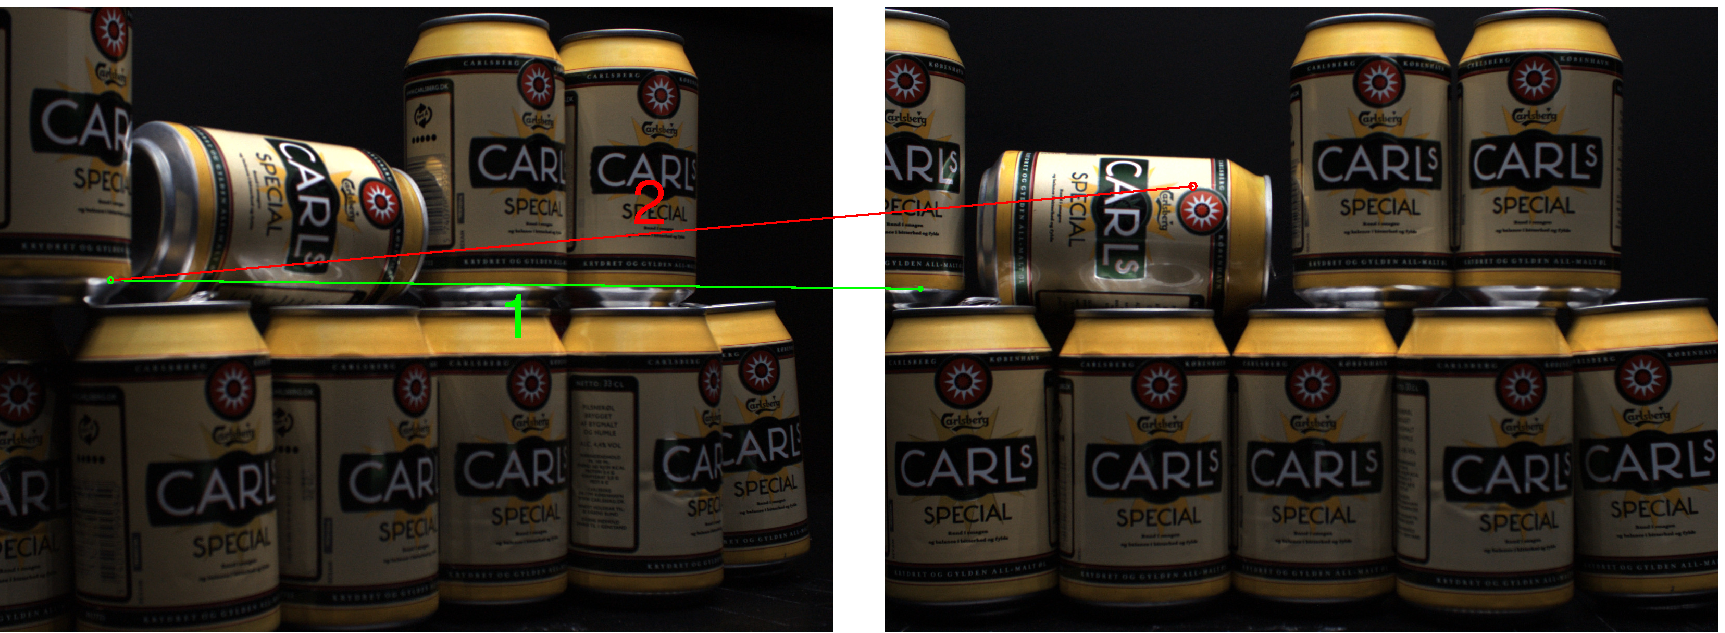
\includegraphics[width=\textwidth]{img/imageCorrespondenceCorrectMatch.pdf}
	\caption{Example of a condition positive match. First and second best matches have descriptor distances $0.076$ and $0.083$, respectively, resulting in a distance ratio of $0.92$.}
	\label{fig:imageCorrespondenceCorrectMatch}
	\vspace{5mm}
	%
	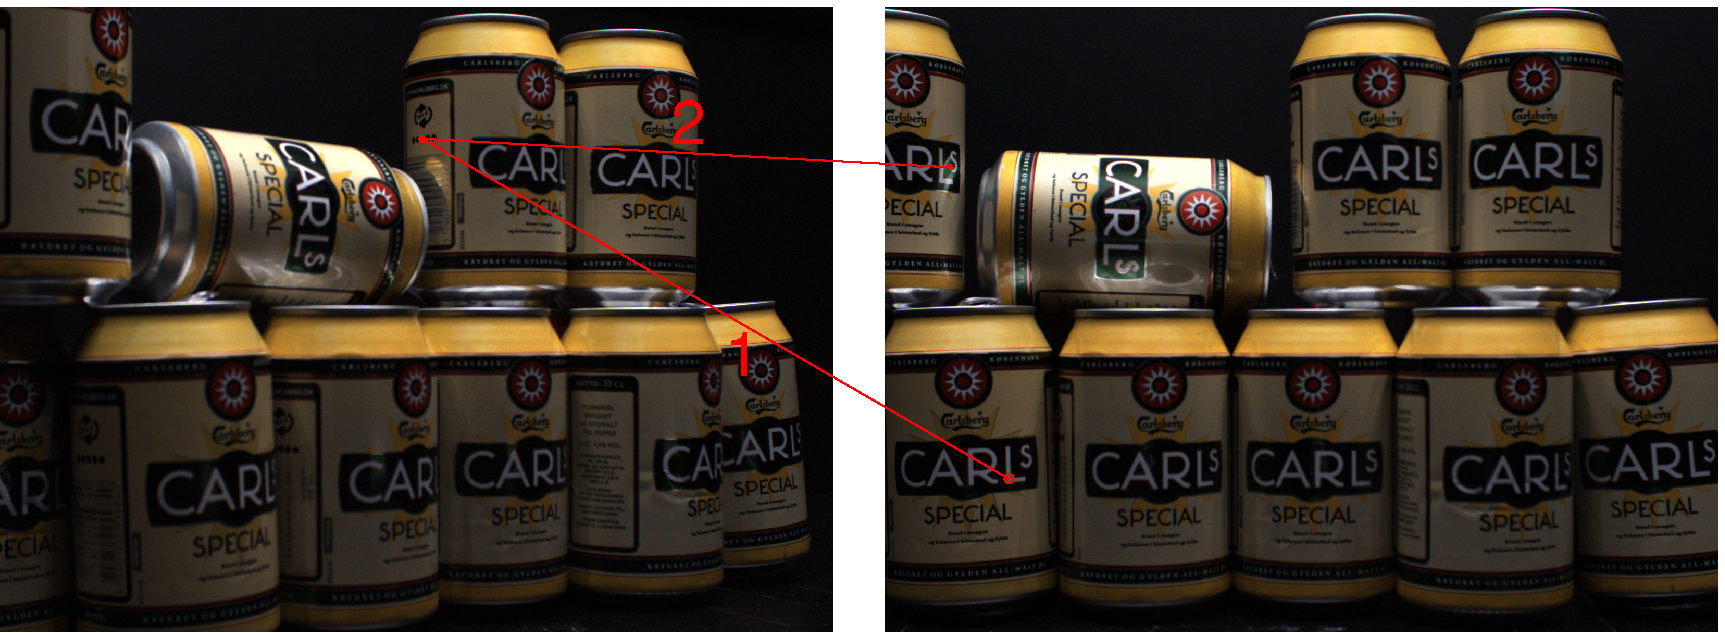
\includegraphics[width=\textwidth]{img/imageCorrespondenceIncorrectMatch.pdf}
	\caption{Example of an condition negative match. First and second best matches have descriptor distances $0.079$ and $0.081$, respectively, resulting in a distance ratio of $0.97$.}
	\label{fig:imageCorrespondenceIncorrectMatch}
\end{figure}
\restoregeometry
%
\begin{figure}[tb]
	\centering
	\begin{subfigure}[t]{0.49\textwidth}
		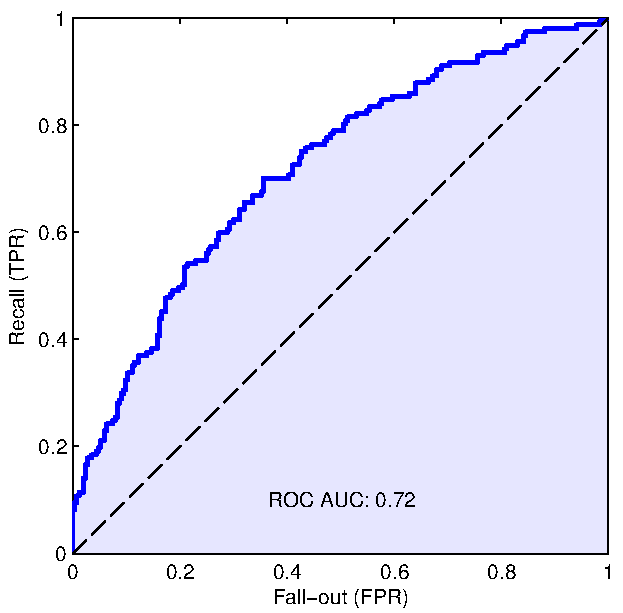
\includegraphics[width=\textwidth]{img/imageCorrespondenceROC.pdf}
		\caption{ROC-curve (blue line), curve of no predictive value attained by classifying randomly (dashed line), and area under the ROC-curve (light blue area)}
		\label{fig:imageCorrespondenceROC}
	\end{subfigure}
	\begin{subfigure}[t]{0.49\textwidth}
		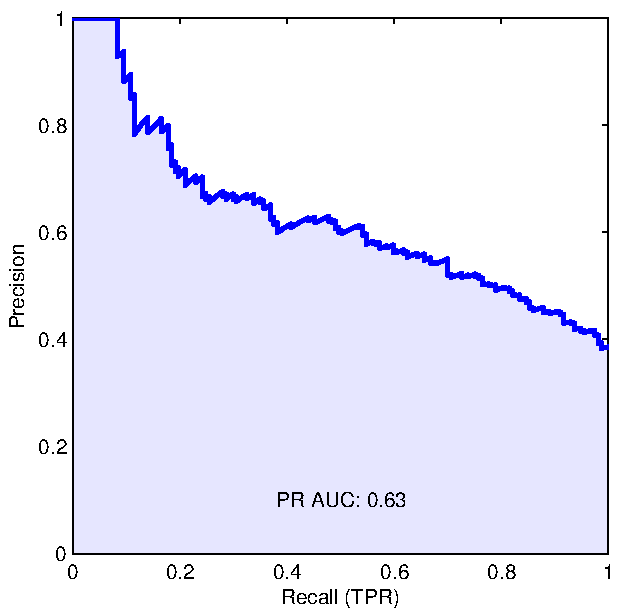
\includegraphics[width=\textwidth]{img/imageCorrespondencePR.pdf}
		\caption{PR-curve (blue line), area under the PR-curve (light blue area)}
		\label{fig:imageCorrespondencePR}
	\end{subfigure}
	\caption{Examples of evaluation measure curves}
	\label{fig:imageCorrespondenceCurves}
\end{figure}
%
\section{Experimental setup}
%
%
\section{Parameter study}
\label{sec:icParameterStudy}
%
We wish to optimize the following parameters:
%
\begin{itemize}
\item Grid type
\item Grid size
\item Grid radius $r$
\item Center scale $\rho$
\item Cell scale $\alpha$
\item Normalization scale $\eta$
\item Bin scale $\beta$
\item Bin count $n$
\end{itemize}
%
\begin{table}[tb]
\centering
\pgfplotstableset{
    highlight/.append style={
        postproc cell content/.append code={
                \pgfkeysalso{@cell content=\textbf{##1}}%
        },
    }
}
\pgfplotstableread[col sep=comma]{../src/results/DTUparamsGo.csv}\loadedtable
\pgfplotstabletranspose[colnames from=Row]{\loadedtable}\loadedtable
\pgfplotstabletypeset[
	string type,
	every head row/.style={
		before row={%
			 {} & \multicolumn{6}{c|}{Splits} & {} \\
			},
		after row={\hline}
	},
%	every last row/.style={after row=\hline},
    columns/colnames/.style={
        string type,
        column name={Variable},
        column type={l|}
    },
    every last column/.append style={
    	column type={|c},
    	highlight
    },
    col sep=comma
]\loadedtable
\caption{Parameter study optimal parameters from 6-fold cross validation using gradient orientation as bin value and gradient magnitude as magnitude type}
\label{fig:ICparamsGo}

\pgfplotstableread[col sep=comma]{../src/results/DTUparamsSi.csv}\loadedtable
\pgfplotstabletranspose[colnames from=Row]{\loadedtable}\loadedtable
\pgfplotstabletypeset[
	string type,
	every head row/.style={
		before row={%
			 {} & \multicolumn{6}{c|}{Splits} & {} \\
			},
		after row={\hline}
	},
%	every last row/.style={after row=\hline},
    columns/colnames/.style={
        string type,
        column name={Variable},
        column type={l|}
    },
    every last column/.append style={
    	column type={|c},
    	highlight
    },
    col sep=comma
]\loadedtable
\caption{Parameter study optimal parameters from 6-fold cross validation using shape index as bin value and curvedness as magnitude type}
\label{fig:ICparamsSi}
\end{table}


Test: 6 fold cross validation.
Tune on 5 folds, test on 1.
%
  
%
Notes:

1. Problems with boosting the noise when using pixel normalization?
%
\subbibliography
\end{document}
